\chapter{Theory}
\label{chap:theory}

% \chapterquote{NO FATE BUT THE NARRATIVES WE IMPOSE ON LIFE'S RANDOM CHAOS TO
% DISTRACT OURSELVES FROM OUR EXISTENTIAL PLIGHT}{xkcd 1177}

\section{The Standard Model of particle physics}
\label{sec:sm}

%andrew's thesis looks quite brief and concise
The \acf{SM} describes the interaction of matter through the
electromagnetic, weak nuclear and strong forces in the context of a
renormalisable quantum field theory
\cite{Salam:1964ry,Glashow:1961tr,PhysRevLett.19.1264}. The matter
particles are represented as spin-$\frac{1}{2}$ fermionic fields and
forces are represented as spin-1 bosonic fields. An additional spin-0
\emph{Higgs} field is included to provide the bosons of the weak force
with their mass. The \SM is built around the concept of local gauge
invariance. When the symmetries of the \SM local gauge group,
$SU(3)\times SU(2) \times U(1)$, are applied to the fermions they
imply the existence of the force carrying bosons. This section will
briefly explore how this leads to the particle phenomenology of the
\SM.

The \SM is typically considered within a lagrangian formalsim. In a
quantum field theory all the the relevant fields and their
interactions are described by a lagrangian density. The lagrangian
density of the \SM can be divided into four parts:
\begin{equation}
\mathcal{L}_{SM}=\mathcal{L}_{gauge}+\mathcal{L}_{fermion}+\mathcal{L}_{Higgs}+\mathcal{L}_{Yukawa},
\end{equation}
$\mathcal{L}_{fermion}$ describes the fermion
fields, their interactions with the bosons are described in
$\mathcal{L}_{gauge}$. The final two terms, $\mathcal{L}_{Higgs}$ and
$\mathcal{L}_{Yukawa}$, describe how the particles within the \SM
obtain mass through interactions with the Higgs field.

Throughout this section the convention $c=\hbar = 1$ is used and the
Einstein four-vector summation convention is assumed. Four-vector indices
are labelled as $\mu$ and $\nu$.

\subsection{The fundamental particles}

The fundamental particles of the \SM comprise fermions and the force
mediating bosons, a summary of them and their relevant
electromagnetic, weak and strong force charges can be seen in
Table~\ref{tab:smParticles}. 

The fermions consist of three generations of charged leptons and their
corresponding weak force partner, the neutrinos. There are
additionally three generations of up-quarks and down-quarks. For all
of these twelve fermions there are corresponding antiparticles that
have the same mass but opposite quantum numbers. As fermions are
spin-$\frac{1}{2}$ particles they are described by the Dirac equation
\cite{Griffiths:111880}:
\begin{equation}
(i\gamma^{\mu}\partial_{\mu}-m)\psi=0,
\end{equation}
where $\gamma^{\mu}$ are the Dirac matrices, defined by their
anti-commutation relation:
\begin{equation}
\{\gamma^{\mu},\gamma^{\nu}\}=\gamma^{\mu}\gamma^{\nu}+\gamma^{\nu}\gamma^{\mu}=2g^{\mu\nu},
\end{equation}
where $g^{\mu\nu}$ is the Minkowski metric. The covariant derivative is denoted
by $\partial_{\mu}$ and $m$ is the mass of the particle in question.

There are five types of bosons that arise from the \SM gauge
symmetries: photons, gluons, $W^{\pm}$, $Z^0$ and the Higgs. Their
properties will be discussed further in this section.

%\begin{table}[htbp!]
\begin{table}
\begin{tabular}{l|l c|c|c|c|c|c}
%\hline 
Categories & Particle & & Mass & Spin & Electric & Colour & Weak \\
 &  & & & & charge & charge & isospin ($t_3$)\\
\hline
\hline
Leptons & electron & $e$ & 0.511~MeV & & & & \\
                & muon & $\mu$ & 106~MeV & $\frac{1}{2}$ & -1  & 0 &  $-\frac{1}{2}$\\
                & tau & $\tau$ & 1777~MeV  & &   &  &  \\
\hline
Neutrinos & electron & $\nu_e$ & <225~eV & & & & \\
                & muon & $\nu_{\mu}$ & <0.19~MeV & $\frac{1}{2}$  & 0  & 0 &  $+\frac{1}{2}$\\
                & tau & $\nu_{\tau}$ & <18.2~MeV &  &   &  &  \\
\hline
Up- & up & $u$ & 2.3~MeV & & & \\
type      & charm & $c$ & 1.28~GeV & $\frac{1}{2}$ & $+\frac{2}{3}$  & $r,g,b$ &  $+\frac{1}{2}$\\
quarks          & top & $t$ & 173~GeV  &   &  &  \\
\hline
Down-  & down & $d$ & 4.8~MeV & & & & \\
type & strange & $s$ & 95~MeV & $\frac{1}{2}$ & $-\frac{1}{3}$  & $r,g,b$ &  $-\frac{1}{2}$\\
quarks            & bottom & $b$ & 4.18~GeV &  &   &  &  \\
\hline
Force & photon & $\gamma$ & 0 & 1 & 0 & 0 & 0 \\
\cline{2-8}
 mediating &  &  &  &  &  & $r\bar{g},r\bar{b},g\bar{r},g\bar{b}$\\
 bosons & gluon & $g$ & 0 & 1 & 0 & $b\bar{r},b\bar{g},
\frac{1}{\sqrt{2}}(r\bar{r}-g\bar{g})$ & 0 \\
 & &  &  &  &  & $\frac{1}{\sqrt{6}}(r\bar{r}+g\bar{g}-2b\bar{b})$ &  \\
\cline{2-8}
 & W & $W^{\pm}$ & 80.4~GeV &  & $\pm 1$ &  & $\pm 1$ \\
 & Z & $Z^0$ & 91.2~GeV & 1 & 0 & 0 & 0 \\
 & Higgs & $h^0$ & 125~GeV &  & 0 &  & $-\frac{1}{2}$ \\
%\hline
\end{tabular}
\caption{All the fundamental Standard Model fermions and bosons and
their charges \cite{PhysRevD.86.010001}}
\label{tab:smParticles}
\end{table}

\subsection{Gauge symmetries}
\label{sec:gaugeSymmetries}

The insensitivity to the structure of a theory to a specific
transformation constitutes a symmetry. This concept is very powerful
for gaining insights into fundamental physical theories. For example,
the fact that physical laws do not change over time,
time-translational symmetry, leads to the conservation of energy.  In
general, any symmetries have a corresponding conserved quantity, as
laid out in Noether's theorem \cite{1971TTSP....1..186N}. This concept
is used extensively when formulating the \SM and allows for the
derivation of observed interactions through the imposition of a few,
fairly straightforward, symmetries.

The effect of applying a symmetry within the \SM is demonstrated when
imposing local $U(1)$ invariance on the Dirac lagrangian for a
fermion, with wavefunction $\psi$ and mass $m$ \cite{Griffiths:111880}:
\begin{equation}
\mathcal{L}=i\bar{\psi}\cancel{\partial}\psi-m\bar{\psi}\psi.
\end{equation}
A global $U(1)$ transformation, $\psi\rightarrow e^{iq\theta}\psi$,
where the phase $\theta$ and $q$ are constant,
leaves the lagrangian invariant. If this $U(1)$ transformation is
local, i.e. the phase depends on spacetime position, $x$, then the
lagrangian is no longer invariant. It now transforms as:
\begin{equation}
\label{eq:uninvariance}
\mathcal{L}\rightarrow\mathcal{L}-q(\partial_{\mu}\theta(x))\bar{\psi}\gamma^{\mu}\psi.
\end{equation}
However, one can add a vector field, $A_{\mu}$, that interacts with
the fermion field through the lagrangian term:
\begin{equation}
\mathcal{L}_{int}=q(\bar{\psi}\gamma^{\mu}\psi) A_{\mu},
\end{equation}
This vector field is chosen to transform as $A_{\mu}\rightarrow
A_{\mu}+\partial_{\mu}\theta$ and is known as a \emph{gauge field} or
\emph{gauge boson}. The interaction lagrangian term then transforms
under a local gauge transformation as:
\begin{equation}
\mathcal{L}_{int}\rightarrow \mathcal{L}_{int}+q(\partial_{\mu}\theta)\bar{\psi}\gamma^{\mu}\psi,
\end{equation}
this cancels out the term that violated local gauge invariance in
Equation~\ref{eq:uninvariance}. The existence of a new gauge field
allows the addition of an additional gauge invariant term containing
the field strength tensor of the vector field, $F_{\mu\nu}$, which can
be written in general as:
\begin{equation}
F_{\mu\nu}^a=\partial_{\mu}A_{\nu}^a-\partial_{\nu}A_{\mu}^a+gf_{abc}A_{\mu}^{b}A_{\nu}^{c},
\end{equation}
for a general gauge group with the structure constants $f^{abc}$ and
self-coupling constant $g$. For
the $U(1)$ group there is only one self-commuting generator so the
structure constant is 0. For non-Abelian gauge groups, such as
$SU(3)$, the structure constants can be non-zero, which introduces
self interaction terms within the lagrangian. In this case the gauge
boson will carry a charge and can interact with itself.

The final lagrangian for a Dirac fermion can then be written as:
\begin{equation}
  \label{eq:localdiraclagrangian}
  \mathcal{L}=i\bar{\psi}\gamma^{\mu}\mathcal{D}_{\mu}\psi-m\bar{\psi}\psi-\frac{1}{4}F_{\mu\nu}F^{\mu\nu},
\end{equation}
where $\mathcal{D}_{\mu}=\partial_{\mu}+iqA_{\mu}$ and is known as the
\emph{covariant derivative}. This lagrangian will be invariant under
local $U(1)$ transformations. In this case, the addition of one extra
gauge field maintains local invariance as $U(1)$ transformations have
one degree of freedom, corresponding to a generator of the group.
The local gauge invariance of symmetries with more degrees of freedom
require the addition of one gauge boson per degree of freedom. 

The general principle of obtaining local gauge invariance method
through gauge bosons is applied with great success to the gauge group
of the \SM. With the choice of an appropriate gauge group,
$SU(3)\times SU(2) \times U(1)$, the bosons that describe the strong,
weak and electromagnetic forces can all be obtained. In the example
demonstrated in this section the final lagrangian
(Eq.~\ref{eq:localdiraclagrangian}) is that which describes \ac{QED},
predicting the massless photon field, $A_{\mu}$, from the $U(1)$ local
gauge invariance of fermions with a coupling strength corresponding to
the electric charge, represented by $q$. % check this!

\subsection{The strong force}

The strong force can be described with the $SU(3)$ gauge group,
resulting in the interaction of quark fields
via eight massless gauge fields, the gluons. This theory is known as \QCD and
the quark fields possess a colour charge, $C=(r,g,b)$. As the
$SU(3)$ group is non-Abelian, the gluons also possess a colour and
anti-colour charge. This leads to gluon-self couplings, which
results in the short range of the strong force. Additionally,
screening effects from virtual gluons, carrying the colour charge,
leads to the phenomena known as \emph{asymptotic freedom}
\cite{PhysRevLett.30.1343}. This is characterised by the strong coupling constant, $\alpha_S$
getting weaker over short ranges, which leads to quarks behaving as if
they are unbound when they are very close but more strongly coupled as
they move part. The fact that $\alpha_s$ can be small makes it very
challenging to calculate \QCD perturbatively using the well known
techniques that work for electromagnetic and weak force calculations.

One important property of the strong force is that quarks are
confined to exist in colour-singlet states. This can lead to either
\emph{mesons} comprising a quark-antiquark pair or \emph{baryons} that are a
triple quark or anti-quark bound state. These different bound states are known
collectively as \emph{hadrons}. Despite being very strongly bound, if
quarks in these states are given significant energy they can be
liberated through the pair production of quark-antiquark pairs. This
process is known as \emph{hadronisation} and occurs when the energy
contained within the gluons binding the quarks more than the energy
contained within the mass of the produced hadron. When this occurs in
the environment of a particle collider, the quarks typically gain a
significant momentum. This causes them to move out of the bound state,
undergoing hadronisation. If the hadrons that are produced also have
significant energy they can also undergo further fragmentation. This
leads to a quark producing a collimated emission of hadrons from
the collision point, known as a \emph{jet}.

\subsection{Electroweak unification}

The electromagnetic and weak forces are described in the \SM by the
symmetry group $SU(2)\times U(1)$. The requirement of local gauge
invariance in the weak sector led to the electromagnetic and weak
forces being unified within this group in a landmark achievement in
the 1960s \cite{Glashow:1961tr,PhysRevLett.19.1264,Salam:1964ry}.

The $SU(2)$ group has three generators, $T_i=\tau_i/2$, where
$i=1,2,3$ and $\tau_i$ are the Pauli spin matrices. As mentioned in
Sec.~\ref{sec:gaugeSymmetries}, each of these generators is manifested
as a gauge field, labelled $W_{\mu}^i$. Within the electroweak theory
these gauge fields only act on the left handed chiral component of the
fermion field, $\psi_L$, where $\psi_L = (1-\gamma_5)\psi$ and
$\gamma^5=i\gamma^0\gamma^1\gamma^2\gamma^3$. This 
\emph{left-handedness} of the electroweak theory leads to the parity violation
that is observed in weak interactions. The charges associated with
these gauge fields are known as \emph{weak isospin} and are denoted
$t_i$. As with the $SU(3)$ group the $SU(2)$ group is non-Abelian and
the gauge bosons are able to interact with themselves.

The $U(1)$ group has a single generator, with an associated gauge
field, $B_{\mu}$. This field interacts with particles that
carry \emph{weak hypercharge}, $Y=2(Q-t_3)$. It is worth noting that this
is a different charge to that of the $U(1)$ group in \ac{QED}, which was
just the electromagnetic charge, $Q$. 
%describe EWK as mark did

The physical gauge bosons observed in experiments on the electroweak
force are obtained by mixing the $W_{\mu}^i$ and $B_{\mu}$ gauge
fields as follows:
\begin{equation}
  \begin{split}
  \PWpm_{\mu}=\frac{1}{\sqrt{2}}\left(\PW^{1}_{\mu}\mp i\PW^{2}_{\mu}\right) \\
  \PZ_{\mu}=\cos\left(\theta_{W}\right)\PW^{3}_{\mu}-\sin\left(\theta_{W}\right)B_{\mu} \\
  A_{\mu}=\sin\left(\theta_{W}\right)\PW^{3}_{\mu}+\cos\left(\theta_{W}\right)B_{\mu},
  \end{split}
\end{equation}
where $A_{\mu}$ is the photon field, $Z_{\mu}$ is the Z boson field
and $W^{\pm}_{\mu}$ are the W boson fields. The Weinberg angle,
$\theta_W$ is given by the coupling strengths of the weak hypercharge
gauge field, $g'$, and the isospin gauge field, $g$:
\begin{equation}
\theta_W = \frac{g}{g^2+g'^2}.
\end{equation}

The $W^{\pm}$ gauge bosons only couple to the left handed component of
the fermion fields. These left-handed components form weak isospin
doublets in both the quark, $Q_L$, and lepton fields $e_L$. The
right-handed components form weak isospin singlets, $Q_R$ and $e_R$
and have $t_3=0$. For the first generation of quarks, the $u$ and $d$
and the first generation of leptons, $e$ and $\nu_e$, the left and
right handed components of the fields are broken down as follows:
\begin{equation}
  \begin{split}
  e_L=\left(\begin{array}{c} \nu_{e~L} \\
  e_L\end{array}\right),~~~
  Q_L=\left(\begin{array}{c} u_L \\
  d_L\end{array}\right),~~~e_R=e_R,~~~Q_R=u_R,d_R,
  \end{split}
\end{equation}
where a subscript $L$ denotes the left-handed component and a
subscript $R$ denotes the right handed component.

Within the quark doublet the charged current interactions of the
$W^{\pm}$ fields act between up and down type quarks. However, the
mass eigenstate of the quarks is not the same as the electroweak
eigenstate. The mixing between these two eigenstates is described by
the \ac{CKM} matrix \cite{Kobayashi:1973fv}. The matrix is diagonally
dominant, meaning the $W^{\pm}$ fields are most likely to produce
interactions of quarks in the same generation, however this allows for
a non-zero intergenerational mixing of the quark fields.

\subsection{Spontaneous symmetry breaking and the Higgs mechanism}

Despite the success of the description of the \SM forces through a
gauge theory, initial iterations did not provide a way for the
fundamental \SM particles to have a gauge invariant mass term in the
lagrangian. This problem was solved through a spontaneous breaking of
the electroweak symmetry that became known as the \emph{Higgs
mechanism}
\cite{Englert:1964et,Higgs:1964ia,Higgs:1964pj,Guralnik:1964eu,Higgs:1966ev,Kibble:1967sv}.
This spontaneous symmetry breaking allowed the vector bosons of the
weak force to obtain mass and provided a way to write gauge invariant
mass terms for the fermions.

A symmetry is spontaneously broken if the ground state of
the vacuum does not share the symmetry of the lagrangian
\cite{Griffiths:111880}. Even though the collection of all states does
share the symmetry, when the theory is in its ground state a
particular vacuum energy must be chosen. This allows terms which are
not gauge invariant to be added to the theory by coupling some of the
fields to a new field with a non-zero vacuum expectation value. This
is achieved within the \SM by introducing a complex scalar $SU(2)$
field with four degrees of freedom, $\phi$, called the Higgs field:
\begin{equation}
\phi=\left(\begin{array}{c}\phi^+ \\ \phi^0 \end{array}\right).
\end{equation}
This is implemented into the theory through an additional term in the
\SM lagrangrian:
\begin{equation}
\mathcal{L}_{Higgs} =
(\mathcal{D}_{\mu}\phi)^{\dag}(\mathcal{D}^{\mu}\phi) - V(\phi),
\end{equation}
where the covariant derivative is chosen to keep the Higgs field
invariant under $SU(2)\times U(1)$ transformations with a weak
hypercharge of $y=\frac{1}{2}$.

% of:
% \begin{equation}
% \mathcal{D}_{\mu}=\partial_{\mu}-\frac{i}{2}g_1W_{\mu}.
% \end{equation}
To spontaneously break the symmetry the potential, $V$, is chosen to
take the form:
\begin{equation}
\label{eq:higgsPot}
V(\phi)=-\mu^{2}\phi^{\dag}\phi+\lambda\left(\phi^{\dag}\phi\right)^{2},
\end{equation}
where $\mu^2>0$ and $\lambda>0$. This leads to a potential with a
non-zero expectation value that forms a circle in phase space. This
leads to a continuous set of equivalent minima of which one must be
chosen, resulting in the spontaneous symmetry breaking. By convention a
particular minimum is chosen as:
\begin{equation}
\bra{0}\phi\ket{0}=\left(\begin{array}{c} 0 \\ \sqrt{\frac{\mu^{2}}{2\lambda}} \end{array}\right)=\frac{1}{\sqrt{2}}\left(\begin{array}{c} 0 \\ v \end{array}\right).
\end{equation}
Perturbations about this vacuum expectation value can be parametrised
in the form of four real scalar fields. However, with an appropriate
choice of gauge, three of these degrees of freedom, known as the
\emph{Goldstone bosons} can be set to zero. This leaves one remaining
field, $H$, and perturbations can be written as:
\begin{equation}
  \phi=\left(\begin{array}{c}0 \\ v+H \end{array}\right).
\end{equation}
This can then be inserted into the lagrangian to obtain at leading
order:
\begin{equation}
  \mathcal{L}=\frac{1}{2}\partial_{\mu}H\partial^{\mu}H-\frac{1}{2}\mu^{2}H^{2}+\frac{v^{2}}{8}\left[g_{2}^{2}W_{\mu}^{+}W^{+\mu}+g_{2}^{2}W_{\mu}^{-}W^{-\mu}+\left(g_{1}^{2}+g_{2}^{2}\right)Z_{\mu}Z^{\mu}\right].
\end{equation}
This provides the weak vector bosons $W_{\mu}^{\pm}$ and $Z_{\mu}$
with mass terms $g_2v/2$ and $\frac{v}{2}\sqrt{g_1^2+g_2^2}$
respectively. This also introduces a massive scalar field, $H$, with a
mass $\sqrt{2\mu^2}$, which is the Higgs boson. The aim of providing
the weak vector bosons with mass in a gauge invariant way has
therefore been achieved with the introduction of a Higgs boson. This
Higgs boson has subsequently been discovered by the ATLAS and \CMS
collaborations with a mass of 125~\gev \cite{1207.7214,1207.7235}.

With the existence of a Higgs field, it is also possible to write
gauge invariant mass terms for the fermion fields. These are known as
\emph{Yukawa terms} and take the form:
\begin{equation}
  \mathcal{L}_{Yuk}=y_{f}\left(\bar{f}_{L}\phi f_{R}+\bar{f}_{R}\phi^{\dag}f_{L}\right),
\end{equation}
where $f_L$ is the left-handed component of the fermionic field and
$f_R$ is the right-handed component. The value $y_f$ is the Yukawa
coupling and leads to a fermion mass of $y_fv/\sqrt{2}$. The magnitude
of the mass of the fermion is therefore determined by how strongly it
couples to the Higgs field.

\subsection{Beyond the Standard Model}
\label{sec:bsm}

The \SM has been incredibly successful in describing the physics we
observe up to the scale of electroweak unification, $O(100)$~\gev. It
describes well the behaviour of most the observed fundamental
particles and all its predictions so far have been verified by
experiments throughout the 20th and 21st centuries. However,
inconsistencies between the \SM and some observations points to issues
with the theory that can only be solved with a more fundamental \BSM
theory. The fact that the \SM also provides no description of gravity,
that would be expected to be consistent with \GR, is a convincing
argument for new physics at the energy scale that gravity becomes
relevant. This energy scale is typically referred to as the
\emph{Planck scale}.

One of the most obvious experimental issues with the \SM is that it
predicts neutrinos to be massless. Within the theory neutrinos are
only produced by the weak force in their left-handed state, without
the presence of a right-handed neutrino one cannot write a Yukawa mass
term.  Experiments, however, have observed that neutrinos do in fact
have a mass as they undergo flavour oscillations as they propagate in
their mass eigenstates \cite{PhysRevLett.87.071301,Fukuda:1998mi}.
This can, however, be included relatively straightforwardly within the
\SM with the addition of seven new parameters
\cite{doi:10.1143/PTP.28.870}.  These include the neutrino masses and
the \ac{PMNS} matrix that describes how the neutrino mass and flavour
eigenstates mix.

As touched upon in Chapter~\ref{chap:introduction} there are other,
more major, problems with the \SM that are unreconcilable within the
theory. A glaring theoretical problem with the \SM becomes apparent
when calculating corrections to the Higgs mass, $m_H$, at the loop
level \cite{Martin:1997ns}. The observable mass of the Higgs boson is
very sensitive to loop contributions from fermion and scalar fields.
Due to the quartic term proportional to $\lambda$ in the Higgs
potential (Eq.~\ref{eq:higgsPot}) the Higgs also interacts with itself
at loop level. If it is assumed that the Higgs couples, even indirectly, to
any of the new physics that exists at energy scales above the \SM then the
correction to the Higgs mass, $\Delta m_H$, are of the order:
\begin{equation}
\Delta m_H^2 \sim \frac{\lambda}{4\pi^2}\Lambda^2+\delta M_H^2,
\end{equation}
where $\Lambda$ is the energy scale of the \BSM physics and additional
loop corrections are contained within $\delta M_H$. If the \BSM
physics does not occur until the Planck scale, then the energy scale
of the new physics must be $\Lambda\sim 10^{19}~\gev$. As the Higgs
mass is observed to be at the electroweak scale, $m_H=125~\gev$, there
must be a very precise cancellation provided by the extra corrections
to the Higgs mass, over $\sim18$ orders of magnitude. This is not
physically forbidden, but results in a \emph{naturalness} problem
within the \SM, as an unexplained cancellation of this order is deemed to
be unnatural. This problem is known as the \emph{hierarchy problem}
and guides the development of \BSM theories. A potential solution can
be obtained by introducing \BSM physics at close to the electroweak scale.

Another problem with the \SM comes through a significant inconsistency
with observational astrophysical data. Studies of cosmological
gravitational effects through the study of the rotations of galaxies
\cite{Kapteyn:1922zz,Oort:436532}, gravitational lensing
\cite{Markevitch:2003at}, the structure of matter distributed through
the universe \cite{2012Natur.487..202D} and measurements of the
\ac{CMB} \cite{Ade:2015xua,0067-0049-180-2-225} imply the existence of
an additional form of matter named \emph{\acf{DM}}. The \SM provides
no viable candidate for \DM consistent with these predictions. As \DM
does not appear to interact strongly with the \SM it must be
weakly-interacting. Additionally, assuming that dark matter was
produced thermally in the early universe, one obtains the correct
abundance of \DM for a $\sim 100~\gev$ particle that interacts via the
weak force, this fact is known as the \emph{WIMP miracle}
\cite{Jungman:1995df}. Attempts to understand the nature of \DM
typically look for it colliding with matter on earth, signatures from
\DM annihilation in space or the production of \DM from \SM collisions
in a particle collider. %maybe put in bullet cluster?

The \SM successfully unifies the electromagnetic and weak forces, but
the strong force is not incorporated. For a full unification, the
coupling constants of all the \SM forces would unify at a high energy
scale known as the \emph{GUT} scale. This extra consideration is
aesthetically appealing and can also help to motivate future \BSM
theories.

One of the final major problems of the \SM is the fact that it does
not account for the observed matter-antimatter asymmetry in the
universe. The \ac{CP} violation within the \SM is not significant
enough to account for the asymmetry that we observe and should be taken
account of in a final \BSM theory.
%g-2?

\section{Supersymmetry}
\label{sec:susy}

The fundamental group of Minkowski spacetime isometries is known as
the \emph{Poincar\'e group} \cite{Poincare1906}. The only possible
remaining extension of this group is a symmetry between bosons, $b$,
and fermions, $f$. This symmetry is postulated to exist in nature
under the name of \emph{\acf{SUSY}} \cite{Martin:1997ns}. This theory
postulates the existence of a supersymmetric partner for every \SM
particle with identical quantum numbers except for a difference in the
spin value of $\frac{1}{2}$. As these \emph{superpartners} have not been
observed yet, they must have a higher mass than their \SM
counterparts. This implies that \SUSY must be a broken symmetry. As
there is considerable freedom in how this symmetry breaking occurs
there exists a series of possible versions of \SUSY. The most popular
and simplest versions of supersymmetry is the \MSSM, introduced in
Sec.~\ref{sec:MSSM}.

Along with being theoretically motivated, \SUSY can fully or partially
solve several of the problems with the \SM discussed in
Sec.~\ref{sec:bsm}. In \SUSY the loop contributions to the mass of the
Higgs are opposite in sign for fermions and scalars. If the partners
of the \SM fermions are \SUSY scalars then the contributions from the
\SM fermions are cancelled out. Provided the mass of \SUSY particles
have a value of $O(1)~\tev$, the hierarchy problem is resolved.
Additionally, many versions of \SUSY contain weakly interacting and
stable \acf{LSP}, which provides an excellent candidate for \DM. The
addition of superpartners also helps to unify the coupling constants
of the gauge groups within the \SM. Without \SUSY the different forces
of the \SM do not unify at a fixed energy scale, however loop
corrections from \SUSY particles results in a complete unification, as
shown in Fig.~\ref{fig:runningCoupling}. This additionally hints at
the existence of a unification of particle physics with \GR at high energy scales.
The existence of \SUSY is indeed a prerequisite for string theory, a
favourite unification candidate.

\begin{figure}
  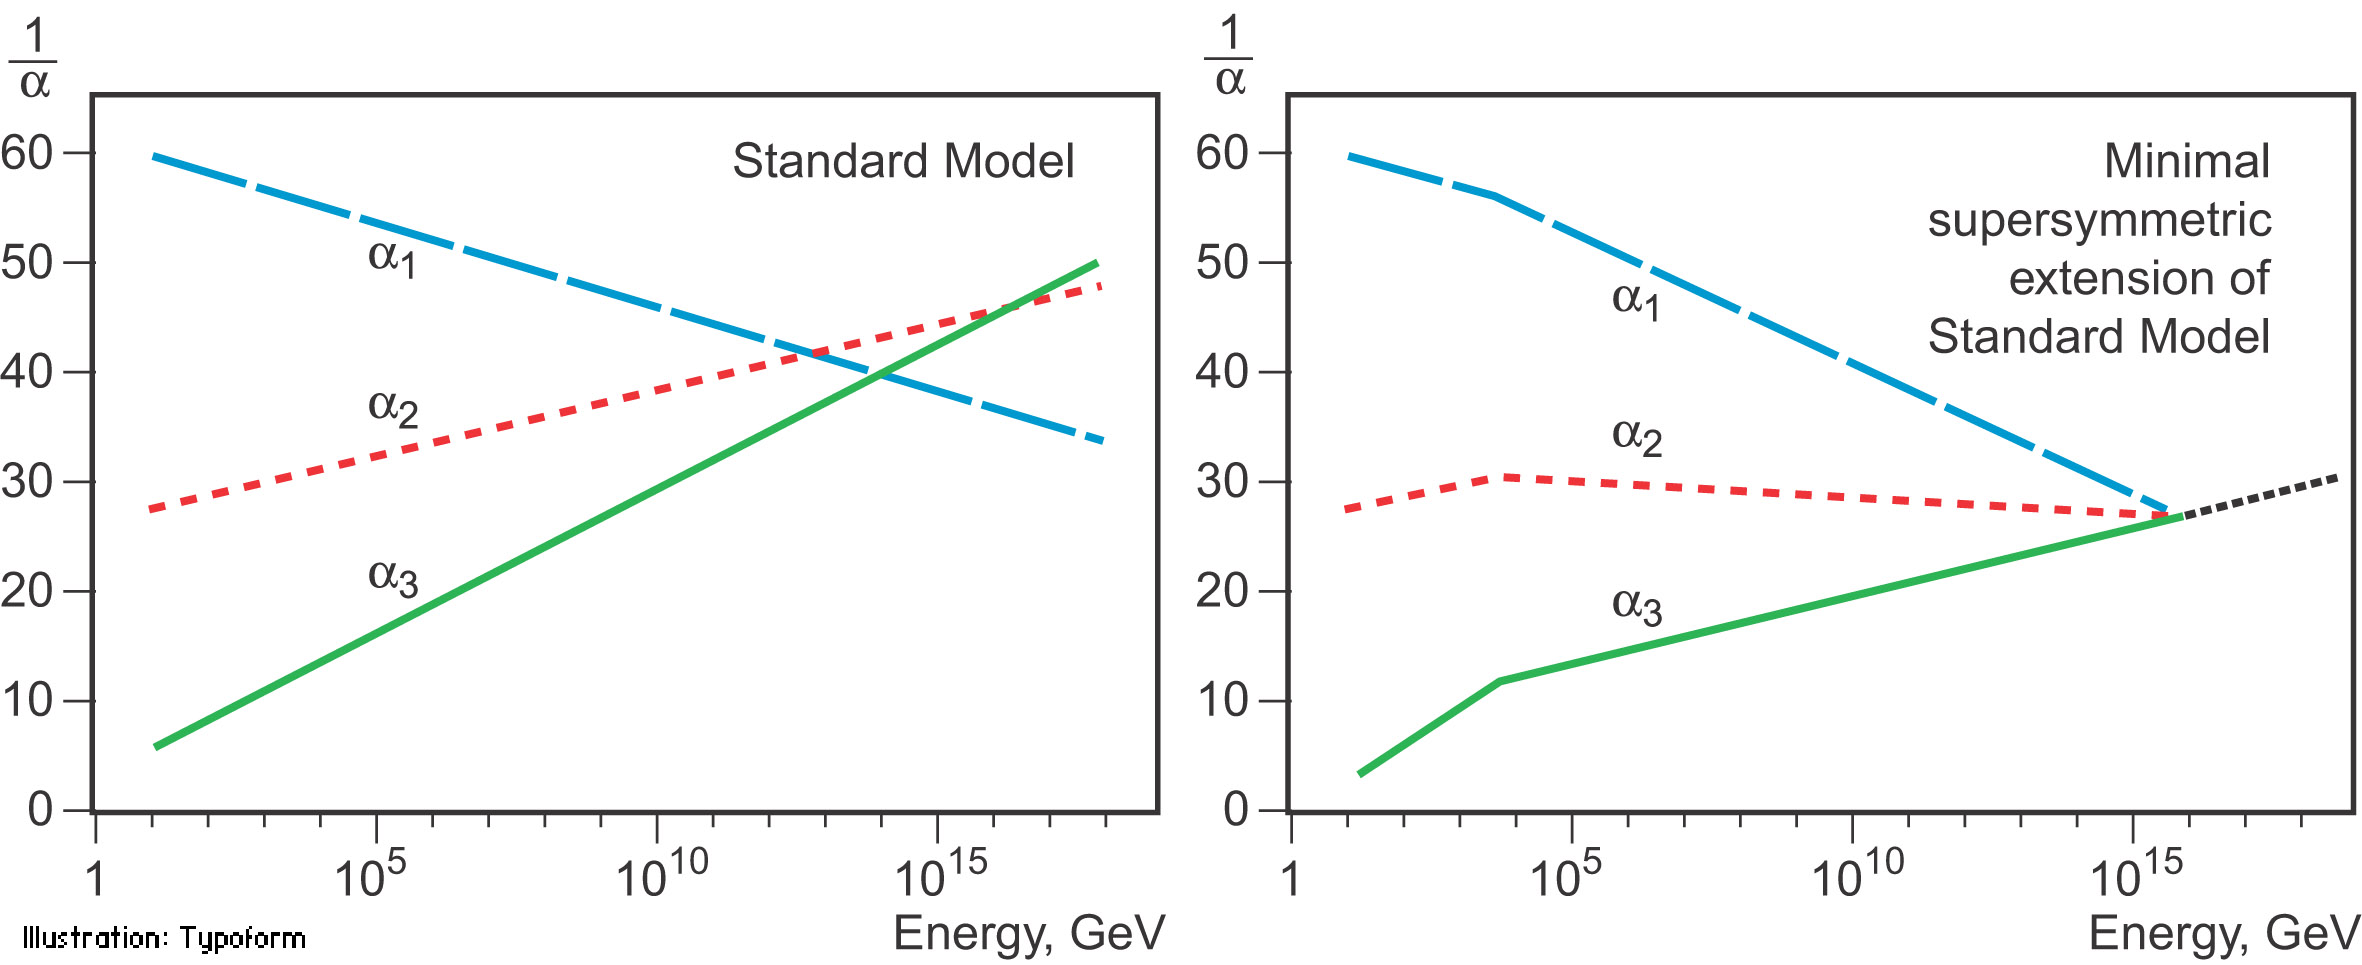
\includegraphics[width=1.0\linewidth]{figs/runningCouplingSusy}
  \caption[]%
  {Evolution of the inverse of the coupling constants of the
  electroweak $U(1)$, $\alpha_1$, electroweak $SU(2)$, $\alpha_2$, and
  strong force $SU(3)$, $\alpha_3$ for the \SM and \MSSM \cite{runningCoupling}}%
  \label{fig:runningCoupling}
\end{figure}

\subsection{The Minimal Supersymmetric Standard Model}
\label{sec:MSSM}

The \acf{MSSM} is a model that incorporates \SUSY with the \SM in a
way that adds the minimum number of new particles and interactions
\cite{Csaki:1996ks}. The \MSSM has 105 free parameters in total, a
significant increase from the 19 in the \SM. A summary of the extra
particles, \emph{sparticles}, introduced by the \MSSM is available in Tab.~\ref{tab:susy}.
The superpartners to the fermions are denoted with the same symbol as
their associated fermion with a tilde above. The weak sector is
extended within the \MSSM and the mixing of the new \SUSY fields
associated to the electroweak and Higgs bosons leads to
the existence of neutralinos, charginos and a total of five Higgs
bosons, including two that carry an electromagnetic charge. 
%Could add in more detail of the fields and things here but it's
%probably not relevant...

\begin{table}
\begin{tabular}{|l|c|c|c|}
%\hline 
Name & Sparticle & Spin & Charge, $Q$ \\
\hline
Up-type squarks & $\tilde{u},\tilde{c},\tilde{t}$ & 0 & $+\frac{2}{3}$ \\
Down-type squarks & $\tilde{d},\tilde{s},\tilde{b}$ & 0 & $-\frac{1}{3}$ \\
Charged sleptons & $\tilde{e},\tilde{\mu},\tilde{\tau}$ & 0 & $\pm1$ \\
Sneutrinos & $\tilde{\nu_{e}},\tilde{\nu_{\mu}},\tilde{\nu_{\tau}}$ & 0 & 0 \\
\hline
%\hline
Gluino & $\tilde{g}$ & $\frac{1}{2}$ & 0 \\
Neutralinos &
$\tilde{\chi_{1}}^0,\tilde{\chi_{2}}^0,\tilde{\chi_{3}}^0,\tilde{\chi_{4}}^0$
& $\frac{1}{2}$ & 0  \\
Charginos & $\tilde{\chi_{1}}^{\pm},\tilde{\chi_{2}}^{\pm}$ &
$\frac{1}{2}$ & $\pm1$ \\
\hline
Neutral Higgs bosons & $h^0,H^0,A^0$ & 0 & 0 \\
Charged higgs bosons & $H^{\pm}$ & 0 & $\pm1$ \\
\end{tabular}
\caption{The extra particles introduced by the \MSSM. The symbol $h^0$
is typically used to denote the \SM Higgs boson.
% A subscript of
% $L$ or $R$ denotes the left or right-handed states respectively
\cite{Martin:1997ns}}
\label{tab:susy}
\end{table}
% table from mark

Unlike the \SM, the \MSSM permits lepton and baryon number violation,
the total numbers of leptons and baryons do not need to be conserved.
This could lead to interactions in which quarks can produce leptons,
such of interactions would allow protons to spontaneously decay.
However, stringent limits have been set on the lifetime of a proton,
$\tau>10^{33}$~years, that should exclude or heavily suppress this
kind of behaviour. This is dealt with in the \MSSM by introducing a
new conserved quantity known as \emph{R-parity}, $R$:
\begin{equation}
R\equiv (-1)^{3(B-L)+2s}
\end{equation}
where $B$ is the baryon number, $L$ the lepton number and $s$ the spin
of the particle. This leads to \SUSY particles having $R=-1$ and \SM
particles have $R=+1$. The consequence of this is that \SUSY particles
always decay to at least one other \SUSY particle. Additionally, any
\SUSY particles produced by \SM interactions must be produced in
pairs and vice versa. With R-parity conservation the \acf{LSP} is
stable. This fact allows it to fulfil the role of \DM in the case that
the \LSP is neutral. In most favoured \SUSY models the \LSP is
therefore typically taken to be a neutralino \cite{Farrar:1978xj}.
% R-parity - put a note on DM
% define lsp - neutralino in the case of DM

For the \MSSM to successfully solve the hierarchy problem an
additional constraint is applied to the \SUSY particles. As there is
no explicit mass hierarchy in the squark generations predicted in
\SUSY, the sparticles of the top-quark, the \emph{stop}, is typically
required to be the lightest of the squarks. This ensures maximal
cancellation of the contributions to the Higgs mass from the
top-quark, which couples most strongly to the Higgs in the \SM.
% light stops - to solve hierarchy problem

\subsection{Signatures of supersymmetry at the \LHC}

Despite the fact that \SUSY presents a promising extension to the \SM
there have been no significant experimental hints of its existence.
Searches for the evidence of \SUSY production have been performed in a
series of particle collider experiments, but have only resulted in
excluding possible regions of \SUSY parameter space. However, for
\SUSY to convincingly solve the hierarchy problem, it is expected to
present itself at the $O(1)$~TeV energy scale. This scale is just
starting to be explored by the \LHC. If \SUSY is to exist in the form
that is typically conceived it should therefore be evident in the
proton collisions produced by the collider.

The fact that there are a lot of different free parameters in the
\MSSM leads to a wide range of possible \SUSY phenomenologies.
However, constraints made by R-parity and naturalness
considerations help to limit the possible signatures. These
constraints typically lead to the pair production of \SUSY particles
that rapidly decay via \SM particles to a weakly interacting neutral \LSP. 
As the produced \SUSY particles have a reasonably high mass, this
leaves a significant missing momentum signature in any detector that
is looking for \SUSY signatures.
% R-parity, naturalness, neutralino lsp make it good for searching

As the \LHC is a hadron collider, the highest cross section \SUSY
production processes occur via the strong force \cite{Martin:1997ns}
\cite{SUSYxsections_NewAspectsof_pp_collisions}. These processes
result in the production of pairs of squarks or gluinos, the \SUSY
particles with colour charge, that predominantly decay via an even
number of \SM quarks to an \LSP. A feynman diagram of typical squark
and gluino production and decay is shown in Fig.~\ref{fig:susyDecay}.
The resulting signature will usually be characterised by high energy
hadronic jets of \SM particles recoiling from invisible particles.

\begin{figure}
  \centering
  \subfloat[]{
    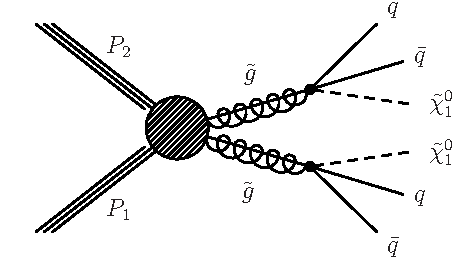
\includegraphics[width=0.4\textwidth]{figs/T1qqqq}
  }~~~ 
  \subfloat[]{
    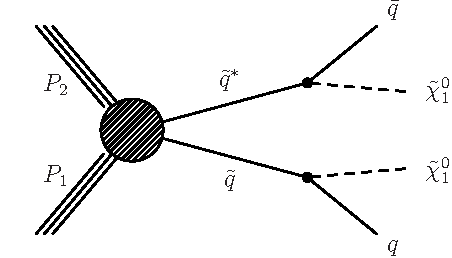
\includegraphics[width=0.4\textwidth]{figs/T2qq}
  }
  \caption{Representative \SUSY production and decay of gluinos, (a), or
  squarks, (b), in proton-proton collisions. The \SUSY particles decay
  to a weakly interacting neutralino, $\tilde{\chi_1}^0$, via \SM
  quarks \cite{smsTwiki}.}
  \label{fig:susyDecay}
\end{figure}

\subsection{Simplified models}

%Decays etc.
